\chapter{Interactive Analysis and Decision Support with MATSim}
\label{ch:businessanalytics}
% ##################################################################################################################

\hfill \textbf{Authors:} Alexander Erath, Pieter Fourie

\begin{center} 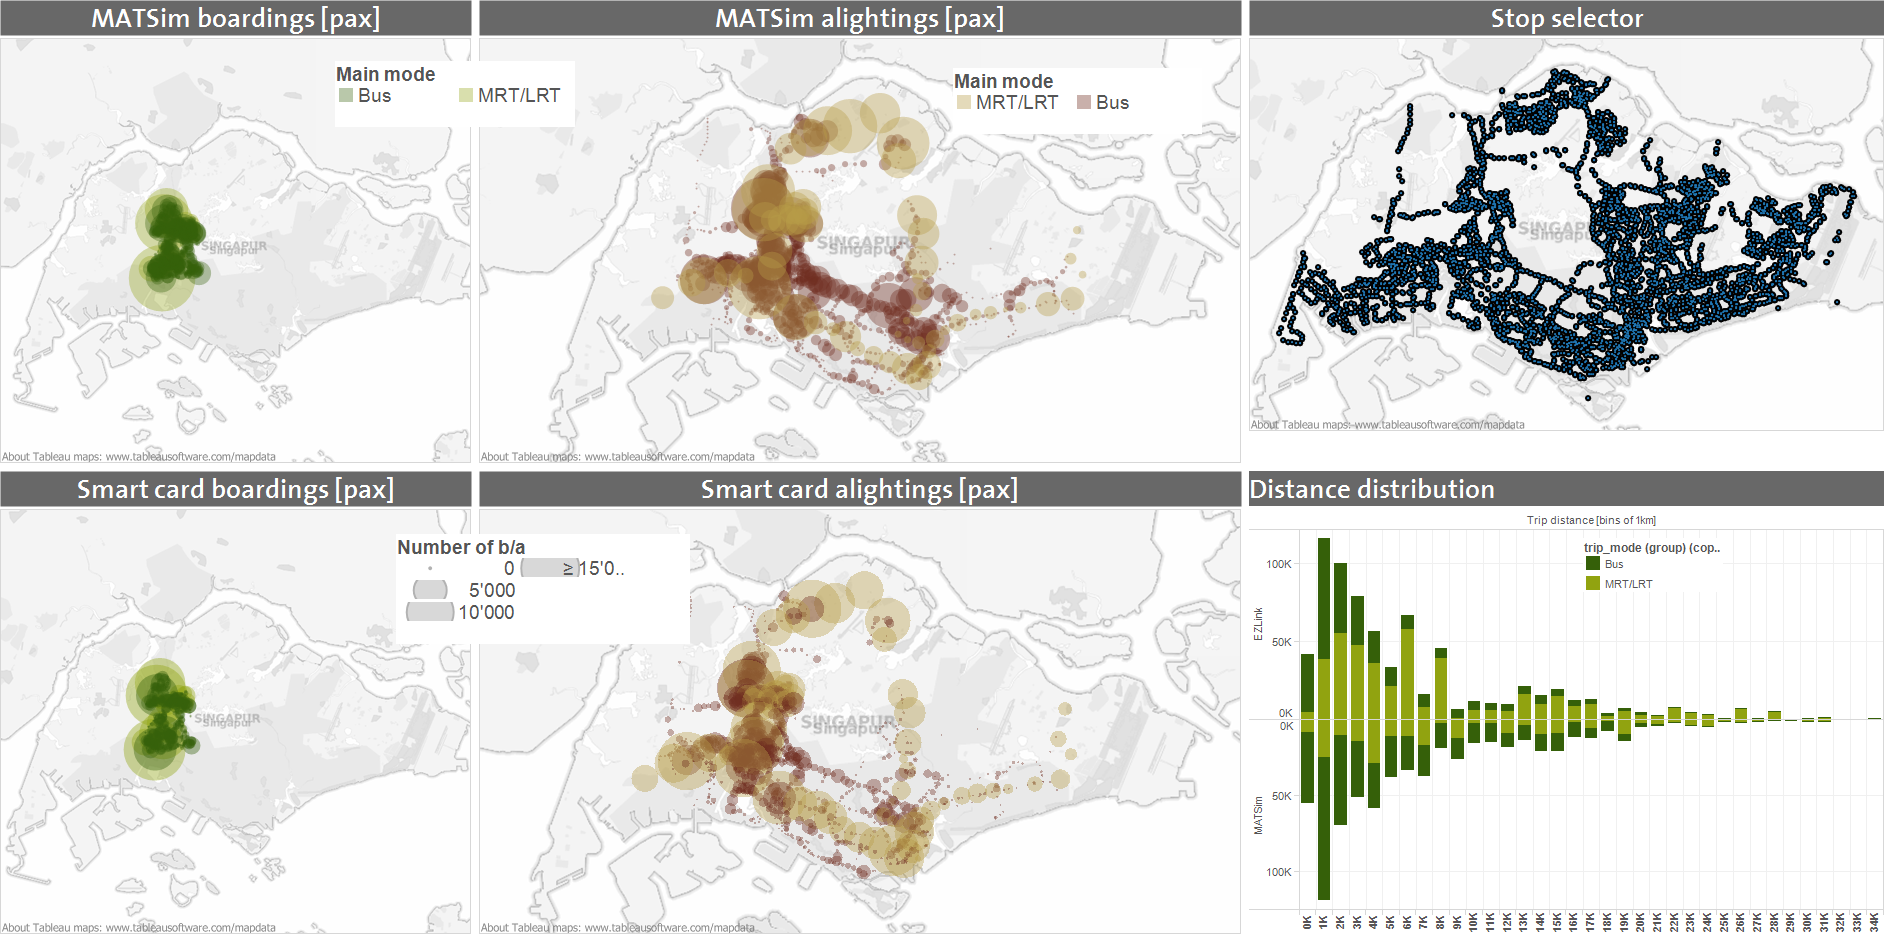
\includegraphics[width=0.4\textwidth, angle=0]{extending/figures/businessanalytics/tableau.png} \end{center}

\editdone{This text has undergone the professional edit. Please no grammatical changes anymore! They are most-probably wrong.}

% ##################################################################################################################


\section{Basic Information}
\createStandardInformationBasic{%
%
\citet{Tableau_Webpage_2013}%
%
}{%
%
Standalone GUI of Tableau Software \citep{Tableau_Webpage_2013} and \lstinline|contrib.analysis.travelsummary| (Section~\ref{sec:contrib-analysis}) for pre-processing
%
}{%
%
in the GUI
%
}{%
%
\citet[][]{ErathEtAl_EASTS_2013}
%
}



% ##################################################################################################################
This chapter is largely based on work in \citet[][]{ErathEtAl_EASTS_2013}, where the interested reader will find references for further reading.
% ##################################################################################################################
\section{Introduction}
\label{sec:analyticsIntro}
% .......................................................
\paragraph{Agent-Based Simulation Means Lots of Data}
Agent-based transport demand models require managing and integrating data sources several orders of magnitude larger than traditional aggregate models. In a truly disaggregate demand description, as seen in our \gls{matsim} implementation for Singapore, spatial data represents individual buildings and land parcels, not zones; travel demand takes the form of a full activity diary with connecting trips for every individual, based on their personal demographic attributes, instead of an aggregate number of trips from zone to zone for a specific time period. For this reason, input data for an aggregate four-step (or related) demand model can generally be edited on a laptop, using standard spreadsheet software, whereas agent-based modeling requires the manipulation and synthesis of large stores of structured, hierarchical data, frequently exceeding most personal computer capacity. %comment

% .......................................................
\paragraph{How MATSim Stores Data}
\gls{matsim} stores and retrieves data from \gls{xml}, because \gls{xml} reflects objects' hierarchical structure in the simulation and is readable. However, performing general exploratory analysis of large \gls{xml} data stores is usually poorly supported by most data analysis software packages, especially \gls{gis}-based systems. To perform analyses, expert knowledge of \gls{xml} querying technologies like XPath and XQuery is required (or \gls{java}, if one performs more specialized analysis on the objects themselves). In our experience, this specialized knowledge is lacking in transport and urban spatial planning practice. Therefore, in most \gls{matsim} applications so far, authorities, and other interested parties, must formulate their desired analysis in advance and have expert consultants perform the analysis. Any queries resulting from the analysis require another consultation cycle and the client's perceived value declines, due to both lack of interactivity and model ownership feeling. We believe this lack of a broadly supported exploratory data analysis interface, and the customer experience the interface can create, presents a considerable barrier to entry for many authorities and operators interested in using \gls{matsim}.

% .......................................................
\paragraph{How Customers Interact With Data: Relational Databases, GUI-Driven Interaction}
Most transport and urban spatial planning customers rely on mature, \gls{gui}-driven software, such as \gls{arcgis} \citep{ARC_GIS_2011}, EMME/3 \citep{EMME_Webpage_2015}, the PTV \citep{PTV_Webpage_2009} transport planning suite, or even Microsoft Excel; all of these connect to relational databases and perform queries on large data sets. Many analysts can explicitly query databases using the \gls{sql}; the \gls{odbc} standard allows software to connect to any relational database regardless of the actual technology driving it. Importantly, many interactive exploratory data analysis software suites, like Tableau, Tibco Spotfire, SAS and the open source R project, support relational databases and \gls{odbc}.

% ##################################################################################################################
\section{Requirements of a Decision Support Interface to MATSim}
\label{sec:analyticsRequirements}
The event stream produced by the \gls{matsim} mobility simulation represents the transport simulation process at the atomic level. It could be fed into a relational database; an analyst fluent in procedural languages could process it in arbitrary ways. But we expect more general use case scenarios, where most analysts will perform general tasks that can be standardized. To this end, we set about compiling requirements specifications for potential audiences and their use case scenarios, to come up with a general interactive analysis framework and decision support to satisfy most requirements. We developed a set of Java classes to process \gls{matsim} input and output, producing tables in a relational database, and an entity relationship diagram that should be intuitive and useful to a large user audience.

% ==============================================================================
\subsection{Users}
This chapter presents a decision support tool geared to decision makers and researchers in the fields of transport planning and operations, spatial planning and spatial economics and geography. Generally speaking, it should serve professionals interested in mobility and spatial analysis, who understand transport modeling principles, but do not have the expertise to operate an agent-based transport simulation directly. Currently, we envision the following stakeholders and some hypothetical questions for a decision-support system---a non-exhaustive list that, we expect, will grow with time:
% .......................................................
\begin{description}\styleDescription
\item[Transport planners:] How many trips occur where, when and what is the activity purpose?
What are the socio-demographic characteristics of people performing these trips and activities?
% .......................................................
\item[Urban Planners:] What are the temporal usage patterns of buildings and the surrounding neighborhood?
What is the flow from public transport stops to surrounding buildings?
% .......................................................
\item[Policy-Makers:] What are the costs and benefits of a new public transport service?
Who are the winners and losers when constructing a new road?
% .......................................................
\item[Public Transport Operators:] What is the breakdown of specific bus lines' ridership?
% .......................................................
\item[Service Industry:] Which customers are in catchment areas, separated by mode?
\end{description}

% ==============================================================================
\subsection{Functional Requirements}
The decision support framework should facilitate classic transport appraisal methods, such as cost/benefit analysis and evaluation of transport infrastructure spatial impact and policy measures. The framework should allow any sort of spatial analysis, on the finest granularity level provided by the transport model; usually, individual buildings or parcels, as well as public transport stops and selected links, like count stations or tolled road segments. However, these geographic features should be indexed against transport zones, or other geographic areas of interes,t to allow customized results aggregation. Furthermore, it should capture all temporal aspects of the simulation; full temporal dynamics are a crucial part of the agent-based approach.

% ##################################################################################################################
\section{General Framework for Decision Support}
Figure~\ref{fig:analyticsFramework} shows the general framework as we envision it: data from various sources feeds into a spatially-enabled database, with all geodata transformed to use the same spatial reference system (ideally, using the same projection used for \gls{matsim} coordinates, allowing for simple distance calculations). Simple \gls{java} programs using the \gls{matsim} \gls{api} and \gls{jdbc} produce \gls{xml} input data for \gls{matsim} scenarios; events from these scenarios are fed back into the database. Analysts query the database to produce ``data cubes'', which are aggregations and queries across many database tables. These are designed for specific purposes, such as calibration and validation, location analysis, winner/loser analysis or other application-specific purposes.

% ==============================================================================
\subsection{Entity Relationship Diagram (ERD) for General Purpose Analysis}
For entity relationships, we decided that a travel diary format is most suitable for the usual types of analysis, but works especially well for comparison with other data sources when validating simulation output. Most travel surveys take the form of a diary, recording travel time, purpose and mode, as well as aspects of the journey like number of stages, transfer walking and waiting time and in-vehicle time. Routines can be developed to transform survey data and public transport smart card records into the same format with consistent coding. Figure~\ref{fig:analyticsERD} shows the \gls{erd} we propose, along with the primary/foreign key relationships between tables that facilitate aggregation and joining of \eg personal/household attributes, such as income, with travel time experienced in the simulation.

% ==============================================================================
\subsection{Interactive Analysis Using Business Analytics Software}
Modern business analytics software, like Tableau \citep{Tableau_Webpage_2013}, provide interactive data aggregation and visualization from relational databases. While basic analysis of individual tables in our proposed \gls{erd} could already provide valuable insight to \gls{matsim} simulations, much richer analysis is possible when tapping relationships between different tables in the database. With the help of graphical query building software, little or no knowledge is required to construct \gls{sql} scripts that create customized data cubes. These cubes are fed into the business analytics software, which is designed with a relatively programming-agnostic audience in mind. Relying on the familiar paradigm of drag-and-drop interaction in a simple, well-documented \gls{gui}, the user constructs ``dashboards'' summarizing information and allowing interactive aggregation, or drilling-down across multiple dimensions.

Figure~\ref{fig:analyticsTableau} shows a Tableau visualization comparing public transport ridership from a \gls{matsim} simulation to actual smart card data records (transformed into the travel diary format specified in the \gls{erd}). Figure~\ref{fig:analyticsJoin} shows the \gls{sql} query used to produce the data frame driving the Tableau analysis. The query exploits the primary/foreign key relationships in the database to perform rapid joins between the different tables.

% ------------
\createfigure%
{General framework of the decision support system}%
{General framework of the decision support system}%
{\label{fig:analyticsFramework}}%
{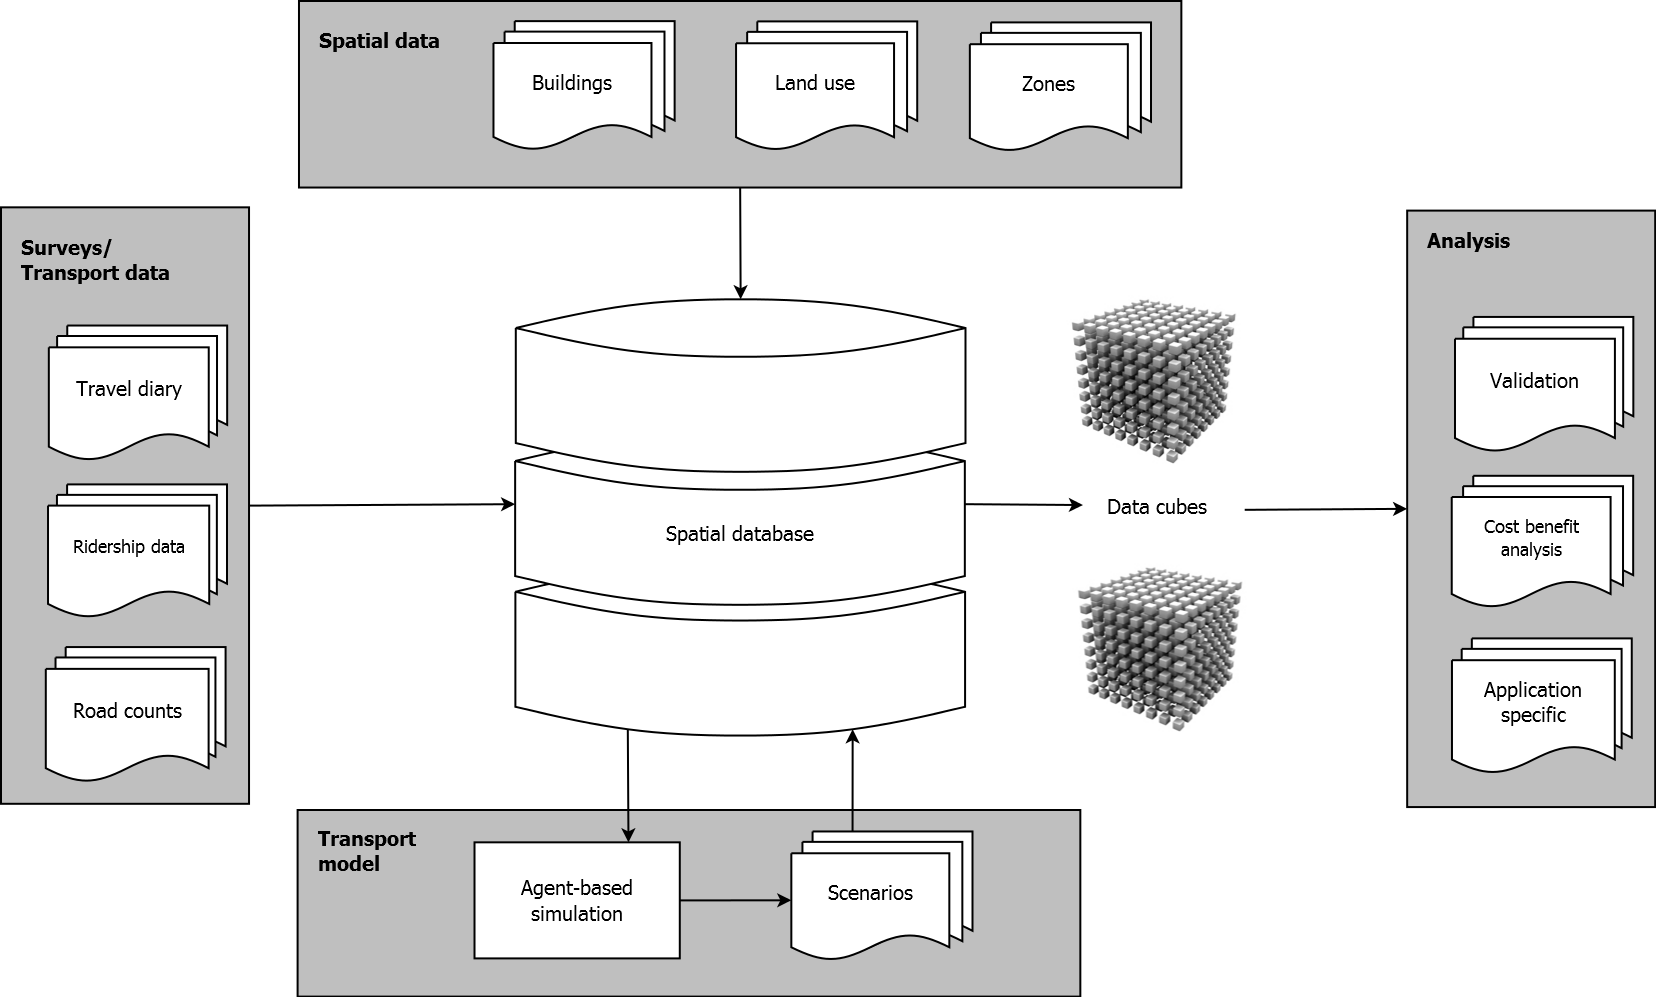
\includegraphics[width=0.65\textwidth, angle=0]{extending/figures/businessanalytics/general}}%
{}
% ------------

% ------------
\createfigure%
{Simplified entity relationship diagram showing shared keys across tables}%
{Simplified entity relationship diagram showing shared keys across tables}%
{\label{fig:analyticsERD}}%
{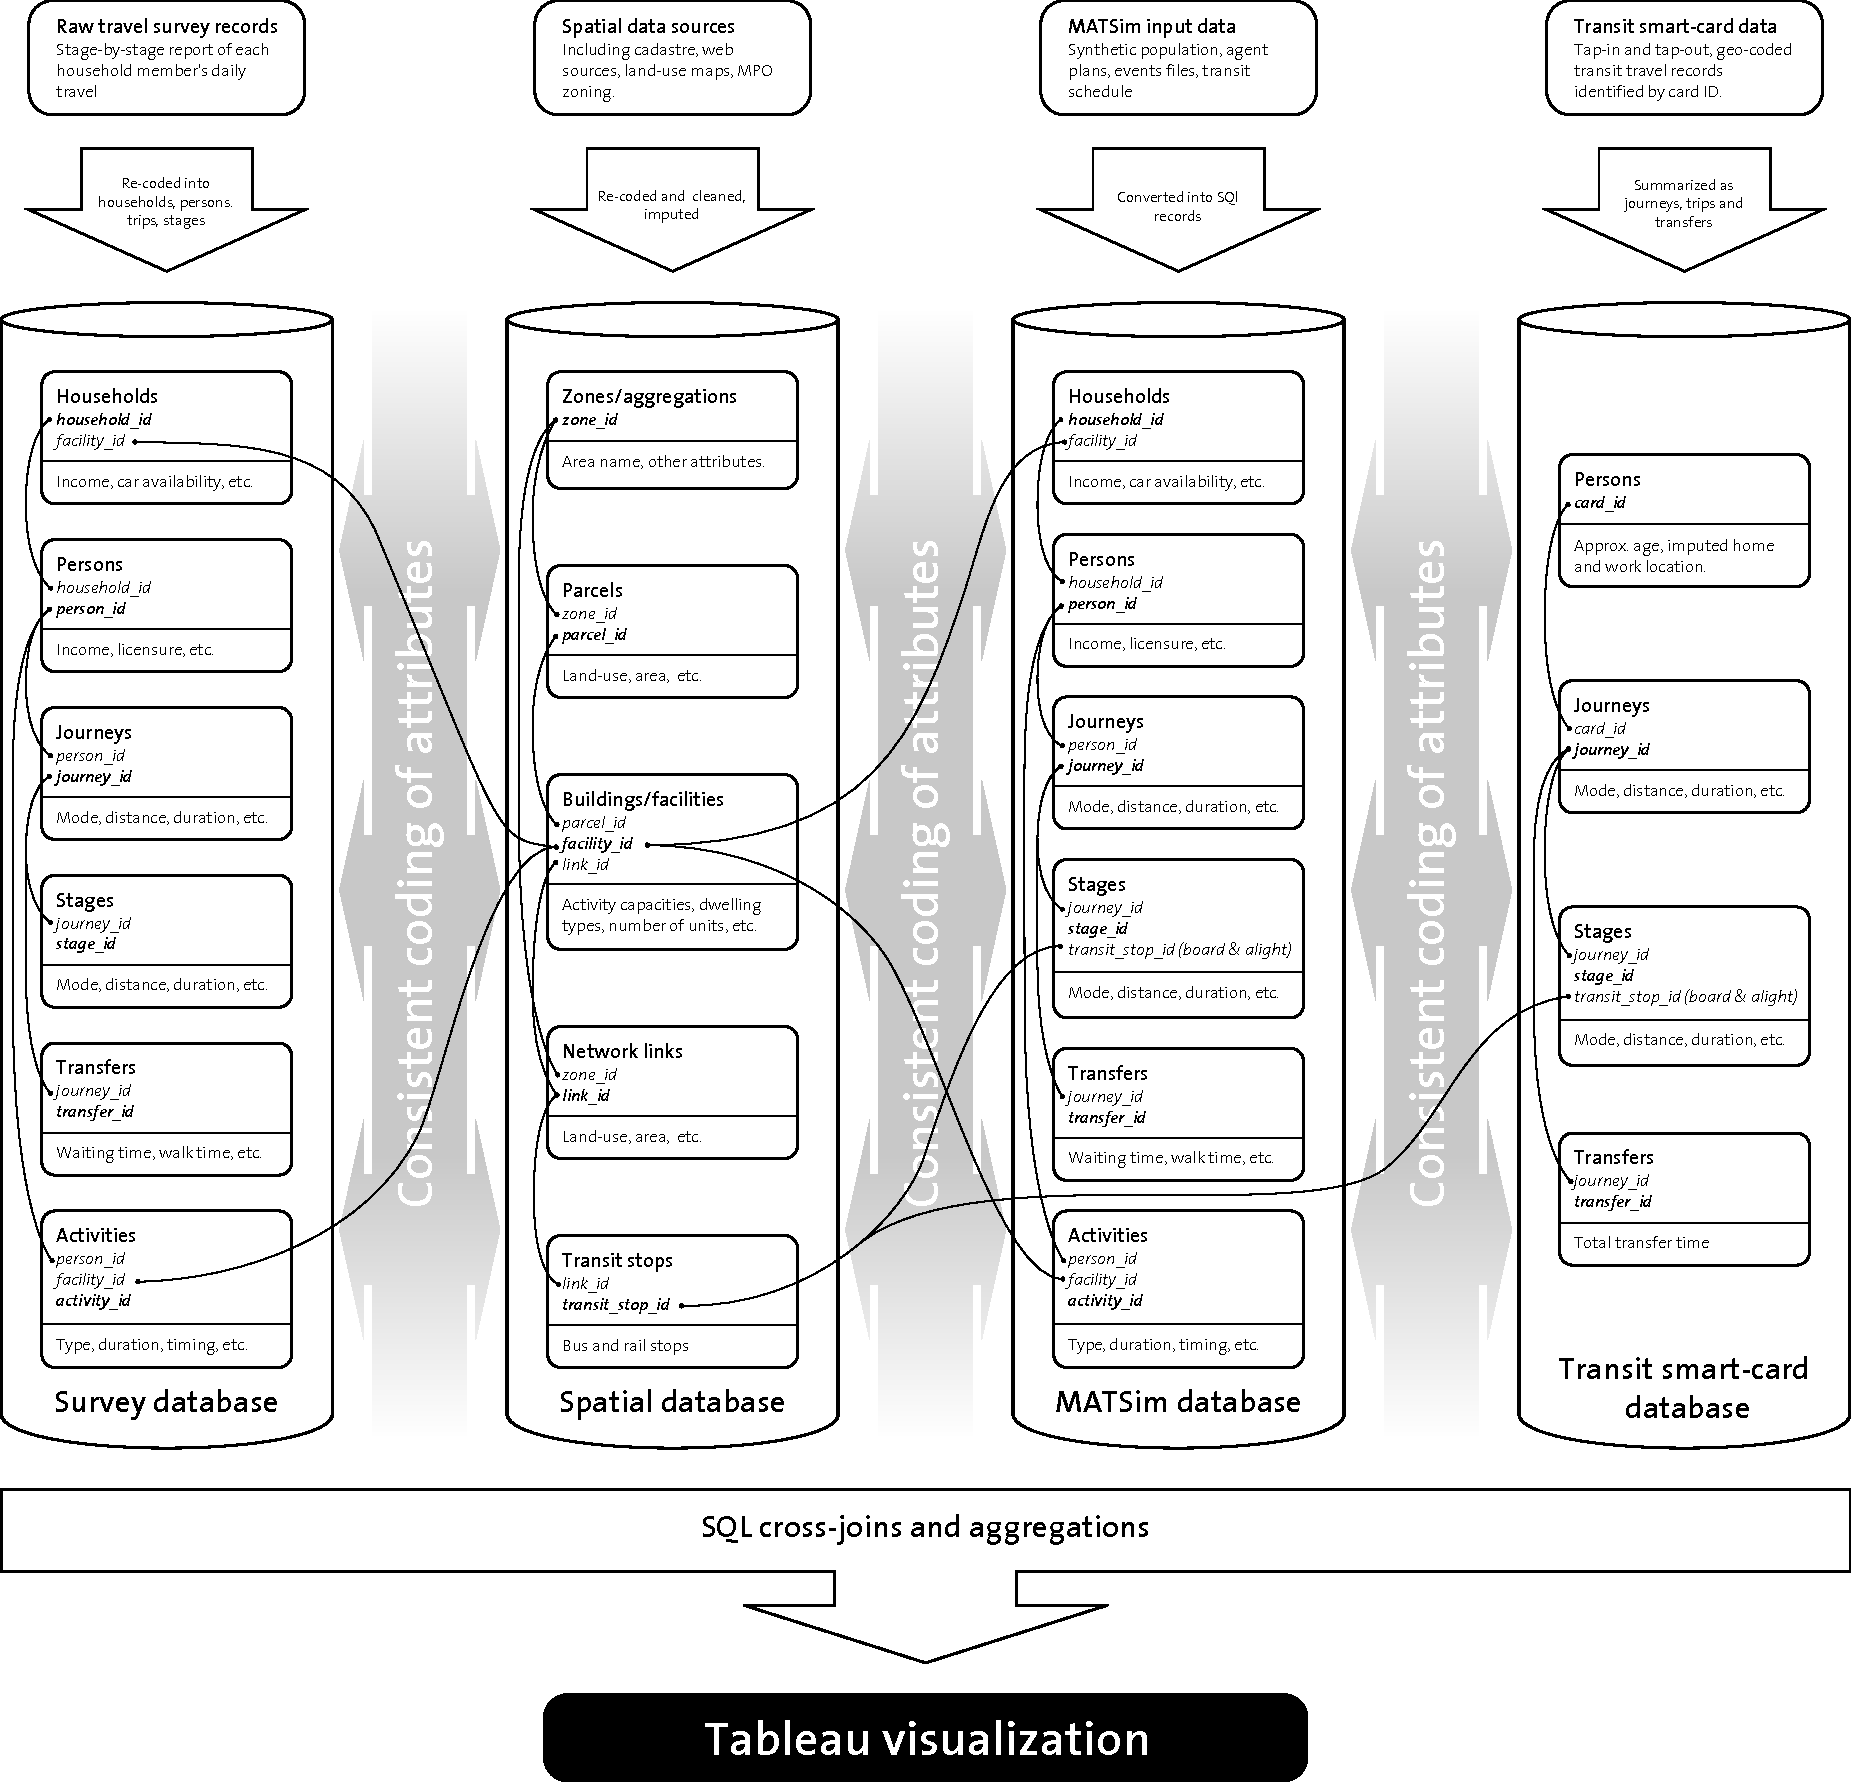
\includegraphics[width=0.65\textwidth, angle=0]{extending/figures/businessanalytics/schema}}%
{}
% ------------

% ------------
\createfigure%
{Tableau visualization}%
{Tableau visualization of public transport ridership from a \protect\gls{matsim} simulation compared against actual smart card data records in Singapore}%
{\label{fig:analyticsTableau}}%
{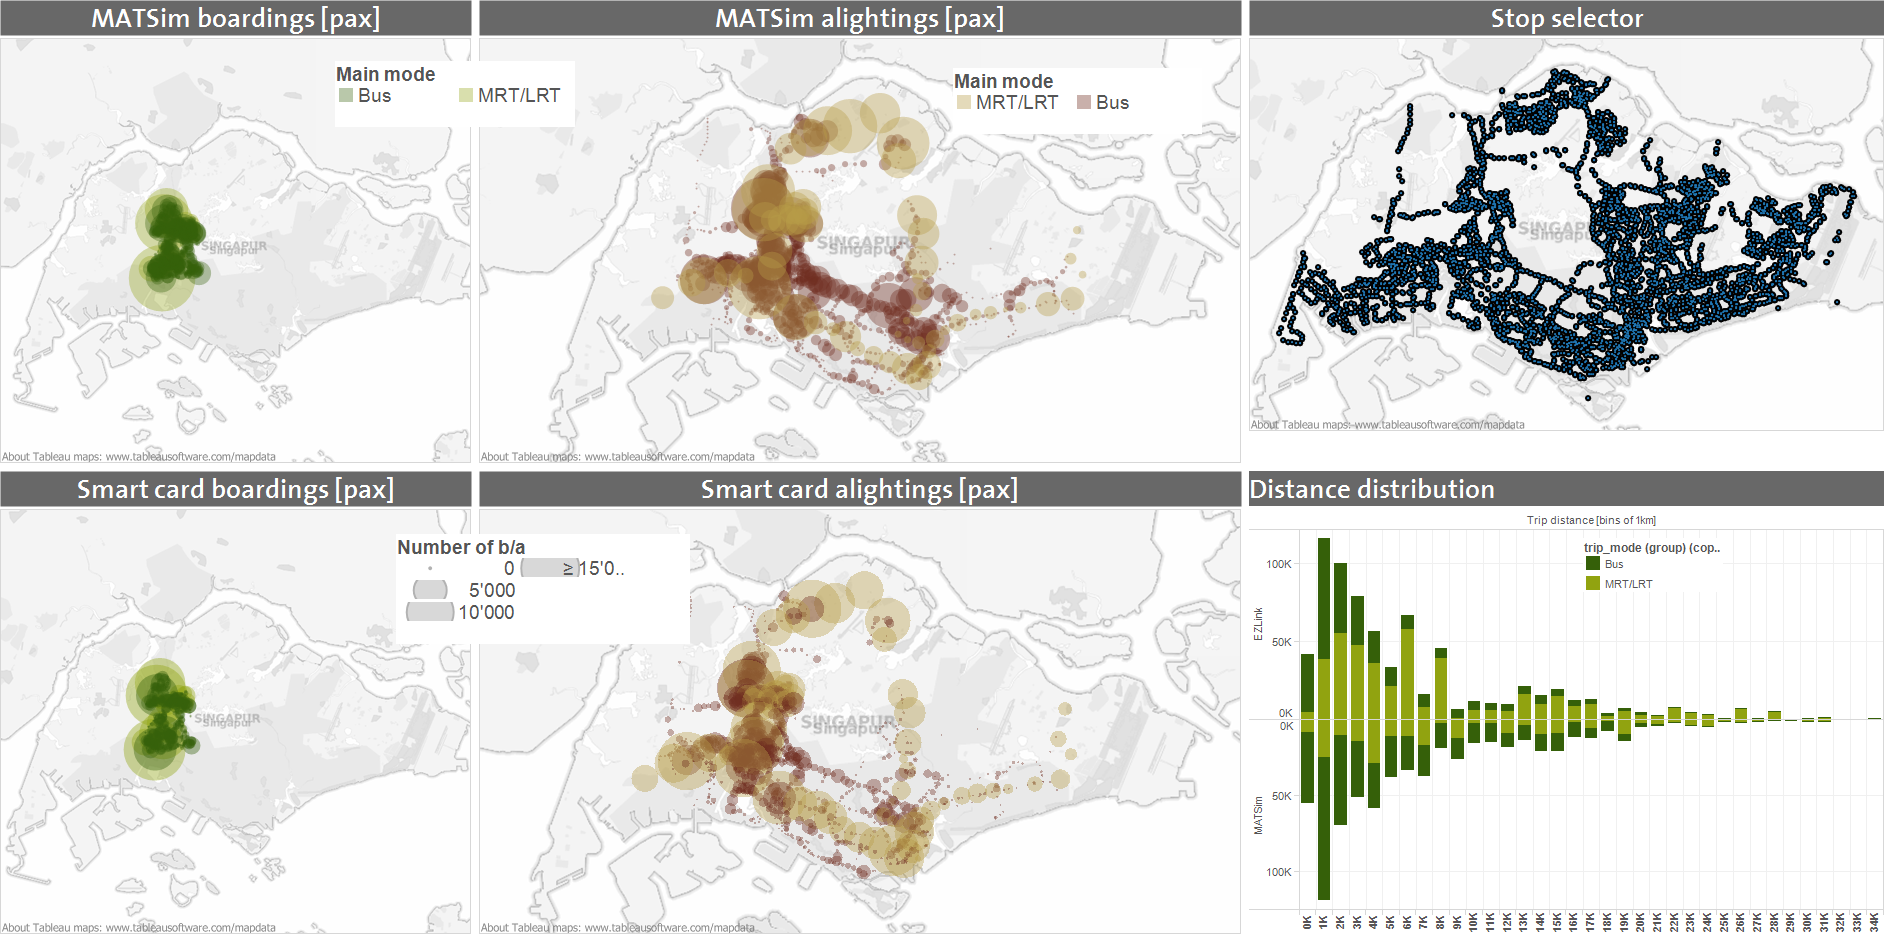
\includegraphics[width=0.65\textwidth, angle=0]{extending/figures/businessanalytics/tableau.png}}%
{}
% ------------

% ------------
\createfigure%
{Table joined in analytics software (Source: \citep{ErathEtAl_EASTS_2013})}%
{A diagram showing how the tables from Figure~\ref{fig:analyticsERD} are joined together for visualization in business analytics software, \eg Tableau, as shown in Figure~\ref{fig:analyticsTableau} (Source: \citep{ErathEtAl_EASTS_2013})}%
{\label{fig:analyticsJoin}}%
{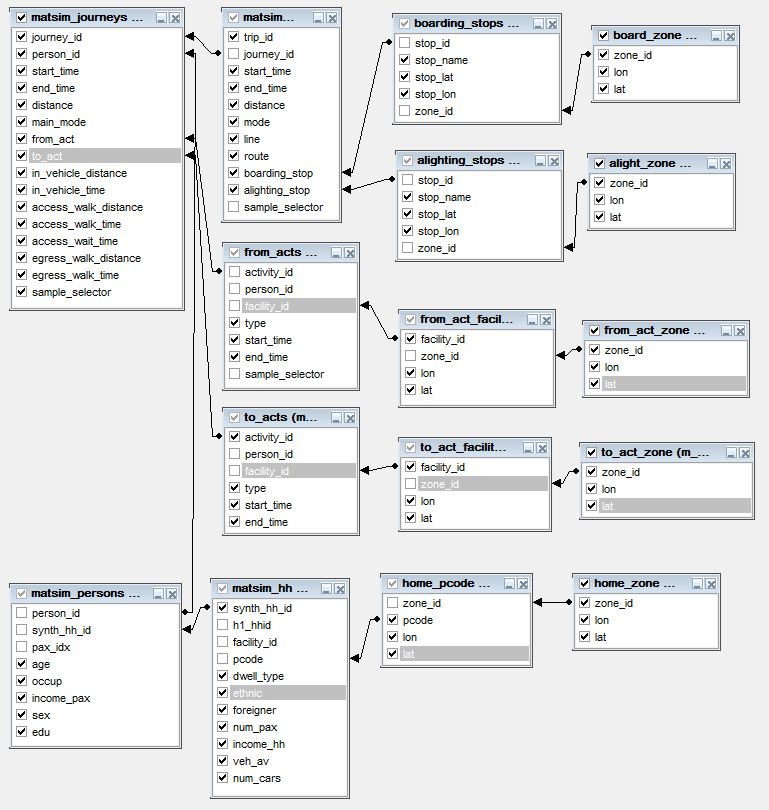
\includegraphics[width=0.65\textwidth, angle=0]{extending/figures/businessanalytics/join}}%
{}
% ------------

% ################################################################################################################
\section{Diaries from Events}
In the package \lstinline|contrib.analysis.travelsummary| (Section~\ref{sec:contrib-analysis}), the reader can find a set of classes that will transform their \gls{matsim} simulation results into a set of travel diary tables, like those discussed in the preceding section. The package contains a simple \gls{gui} class that can be run to specify input data \gls{xml} files, the location to save output \gls{csv} files and other information such as a subscript appended to the end of file names to identify different scenarios. These \gls{csv} files can be read into a relational database of choice, or directly queried in Tableau, or other interactive analysis software.

% ################################################################################################################




% Local Variables:
% mode: latex
% mode: reftex
% mode: visual-line
% TeX-master: "../../main"
% comment-padding: 1
% fill-column: 9999
% End: 
